\documentclass[aspectratio=43]{beamer}

\usepackage{amsmath}
\usepackage{amsfonts}
\usepackage{amssymb}
\usepackage{amsthm}
\usepackage{tikz}
\usepackage{xcolor}
\usepackage{array}
\usepackage{enumitem}
\usepackage{tabularx}

\usetheme{Madrid}
\usecolortheme{default}

\setbeamertemplate{navigation symbols}{}

\setbeamertemplate{footline}{}

\title{}
\author{}
\date{}

\begin{document}
\begin{frame}
\frametitle{Circular arrangements of $\pm 1$'s with total sum 1}

\begin{block}{Lemma}
In any circular arrangement of $\pm 1$'s whose sum is equal to 1, there is
exactly one location starting from which all clockwise partial sums are
positive.
\end{block}

\begin{center}
\begin{tikzpicture}
\draw (0,0) circle (2cm);

\node at (0,2.3) {\small -1};
\node at (1.7,1.7) {\small 1};
\node at (2.3,0) {\small 1};
\node at (1.7,-1.7) {\small -1};
\node at (0,-2.3) {\small 1};
\node at (-0.8,-2) {\small 1};
\node at (-1.8,-1.2) {\small -1};
\node at (-2.2,0) {\small 1};
\node at (-2,1.3) {\small -1};

\end{tikzpicture}
\end{center}

\end{frame}

\begin{frame}
\frametitle{Circular arrangements of $\pm 1$'s with total sum 1}

\begin{block}{Lemma}
In any circular arrangement of $\pm 1$'s whose sum is equal to 1, there is exactly one location starting from which all clockwise partial sums are positive.
\end{block}

\begin{block}{Proof of uniqueness}
If there are two such locations, then the circle breaks into two segments, each summing to $\geq 1$; so the total is $\geq 2$, a contradiction.
\end{block}

\begin{block}{Proof of existence}
Start someplace, find a non-positive partial sum. (If it doesn't exist, we are done.) Start at its end, find a non-positive partial sum, etc. Eventually we must step into a place that has already been visited (after some number of revolutions). It follows that the sum of all entries is $\leq 0$, a contradiction.
\end{block}

\end{frame}

\begin{frame}
\frametitle{Counting paths containing at least one point on the x axis}

\begin{block}{Theorem}
Let $a \geq 1$ and $n \geq k \geq 0$ be integers. The number of paths that
\begin{itemize}
    \item connect the points $(0, a)$ and $(2n, a + 2k)$,
    \item consist of steps with displacement $(1, 1)$ or $(1, -1)$, and
    \item contain at least one point lying on the x axis
\end{itemize}
is equal to $\binom{2n}{n+a+k}$.
\end{block}

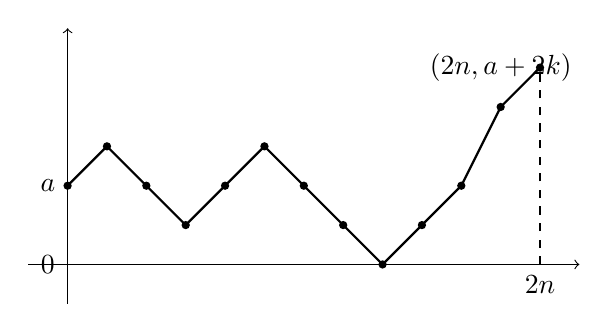
\begin{tikzpicture}[scale=0.5]
    \draw[->] (-1,0) -- (13,0);
    \draw[->] (0,-1) -- (0,6);

    \node at (-0.5, 0) {$0$};
    \node at (-0.5, 2) {$a$};
    \node at (12, -0.5) {$2n$};
    \node at (11, 5) {$(2n, a+2k)$};

    \draw[dashed] (12,0) -- (12,5);

    \draw[thick] (0,2) -- (1,3) -- (2,2) -- (3,1) -- (4,2) -- (5,3) -- (6,2) -- (7,1) -- (8,0) -- (9,1) -- (10,2) -- (11,4) -- (12,5);

    \foreach \point in {(0,2), (1,3), (2,2), (3,1), (4,2), (5,3), (6,2), (7,1), (8,0), (9,1), (10,2), (11,4), (12,5)}
    \fill \point circle (3pt);
\end{tikzpicture}

\end{frame}

\begin{frame}
\frametitle{Counting the Dyck paths}

The Dyck paths of length $2n$ are in bijective correspondence with the ballot sequences of the same length.

\begin{center}
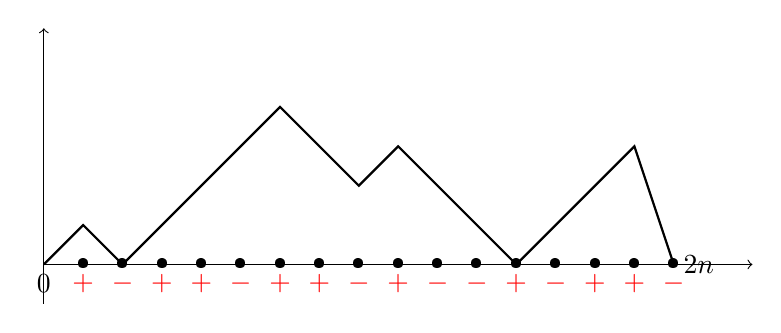
\begin{tikzpicture}
    \draw[->] (0,0) -- (9,0);
    \draw[->] (0,-0.5) -- (0,3);
    \node[below] at (0,0) {$0$};
    \node[right] at (8,0) {$2n$};
    
    \draw[thick] (0,0) -- (0.5,0.5) -- (1,0) -- (1.5,0.5) -- (2,1) -- (2.5,1.5) -- (3,2) -- (3.5,1.5) -- (4,1) -- (4.5,1.5) -- (5,1) -- (5.5,0.5) -- (6,0) -- (6.5,0.5) -- (7,1) -- (7.5,1.5) -- (8,0);
    
    \foreach \x in {0.5, 1, 1.5, 2, 2.5, 3, 3.5, 4, 4.5, 5, 5.5, 6, 6.5, 7, 7.5, 8}
        \node at (\x,0) {\textbullet};

    \node[below,red] at (0.5,0) {$+$};
    \node[below,red] at (1,0) {$-$};
    \node[below,red] at (1.5,0) {$+$};
    \node[below,red] at (2,0) {$+$};
    \node[below,red] at (2.5,0) {$-$};
    \node[below,red] at (3,0) {$+$};
    \node[below,red] at (3.5,0) {$+$};
    \node[below,red] at (4,0) {$-$};
    \node[below,red] at (4.5,0) {$+$};
    \node[below,red] at (5,0) {$-$};
    \node[below,red] at (5.5,0) {$-$};
    \node[below,red] at (6,0) {$+$};
    \node[below,red] at (6.5,0) {$-$};
    \node[below,red] at (7,0) {$+$};
    \node[below,red] at (7.5,0) {$+$};
    \node[below,red] at (8,0) {$-$};

\end{tikzpicture}
\end{center}

\begin{block}{Theorem}
The number of Dyck paths of length $2n$ is $C_n = \frac{1}{n+1} \binom{2n}{n}$.
\end{block}

\begin{block}{Corollary}
The probability that a path $(0,0) \rightarrow (2n, 0)$ consisting of steps of the form $(1, \pm 1)$ is a Dyck path is $\frac{1}{n+1}$.
\end{block}

\end{frame}

\begin{frame}
\frametitle{Counting ballot sequences}

\begin{block}{Lemma}
In any circular arrangement of $\pm 1$'s whose sum is equal to 1, there is
exactly one location starting from which all clockwise partial sums are
positive. Equivalently, there is exactly one entry whose removal
leaves a ballot sequence.
\end{block}

This yields a bijection between ballot sequences of length $2n$ and
circular arrangements of $n + 1$ pluses and $n$ minuses.

The number of such arrangements is $C_n$. We conclude:

\begin{block}{Theorem}
The number of ballot sequences of length $2n$ is $C_n$.
\end{block}

\end{frame}

\begin{frame}
\frametitle{Dyck paths}
\begin{block}{Definition}
A \textcolor{blue}{Dyck path} of length $2n$ is a path in the coordinate plane which
\begin{itemize}
    \item connects the points $(0,0)$ and $(2n, 0)$,
    \item consists of steps with displacement $(1, 1)$ or $(1, -1)$, and
    \item is entirely contained in the upper half-plane $y \geq 0$.
\end{itemize}
\end{block}

\begin{center}
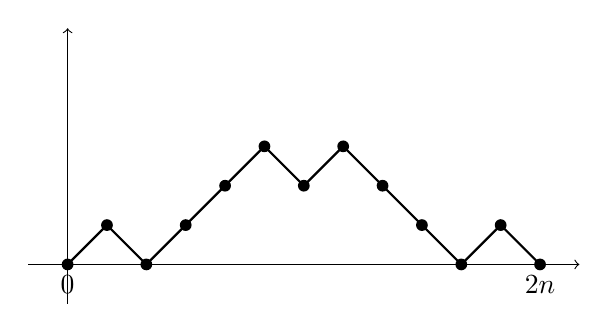
\begin{tikzpicture}[scale=0.5]
    \draw[->] (-1,0) -- (13,0);
    \draw[->] (0,-1) -- (0,6);
    
    \foreach \x in {0,1,2,3,4,5,6,7,8,9,10,11,12}
        \node[circle,fill,inner sep=1.5pt] at (\x, {ifthenelse(\x==0,0,ifthenelse(\x==1,1,ifthenelse(\x==2,0,ifthenelse(\x==3,1,ifthenelse(\x==4,2,ifthenelse(\x==5,3,ifthenelse(\x==6,2,ifthenelse(\x==7,3,ifthenelse(\x==8,2,ifthenelse(\x==9,1,ifthenelse(\x==10,0,ifthenelse(\x==11,1,0))))))))))))}  ) {};

    \draw[thick] (0,0) -- (1,1) -- (2,0) -- (3,1) -- (4,2) -- (5,3) -- (6,2) -- (7,3) -- (8,2) -- (9,1) -- (10,0) -- (11,1) -- (12,0);
    
    \node at (0,-0.5) {$0$};
    \node at (12,-0.5) {$2n$};
\end{tikzpicture}
\end{center}

Dyck paths can be interpreted as trajectories of a random walk on $\mathbb{Z}$ which stay within the nonnegative half-axis.

\end{frame}

\begin{frame}
\frametitle{Alternative way to count the Dyck paths}
Dyck paths are in bijection with the paths $(0, 1) \rightarrow (2n, 1)$ that do
not touch the $x$ axis.

\begin{tikzpicture}[scale=0.7]
    \draw[->] (0,0) -- (10,0);
    \draw[->] (0,0) -- (0,5);

    \node at (-0.2,-0.2) {$0$};
    \node at (9.8,-0.2) {$2n$};

    \foreach \x in {0,1,2,3,4,5,6,7,8,9}
        \node[circle,fill,inner sep=1pt] at (\x, {mod(\x, 2) + 1 + 0.5*sin(deg(\x*2))}) {};

    \foreach \x in {0,1,2,3,4,5,6,7,8}
        \draw (\x, {mod(\x, 2) + 1 + 0.5*sin(deg(\x*2))}) -- (\x+1, {mod(\x+1, 2) + 1 + 0.5*sin(deg((\x+1)*2))});

    \draw[dashed] (9, {mod(9, 2) + 1 + 0.5*sin(deg(9*2))}) -- (9, 0);
\end{tikzpicture}

By the last theorem (with $a = 1$ and $k = 0$), the number of paths
$(0, 1)\rightarrow(2n, 1)$ that touch the $x$ axis is $\binom{2n}{n+1}$. The number of all
paths $(0, 1)\rightarrow(2n, 1)$ is $\binom{2n}{n}$. Hence the number of Dyck paths is
\[
\binom{2n}{n} - \binom{2n}{n+1} = \frac{(2n)!}{n!(n+1)!} \left( \frac{1}{n+1} \right) = \frac{1}{n+1} \binom{2n}{n} = C_n.
\]
\end{frame}

\begin{frame}
\frametitle{The reflection principle}

\begin{block}{Proof}
The set of paths $(0, a) \rightarrow (2n, a + 2k)$ having at least one point on the
$x$ axis is in bijection with the set of \textbf{all} paths $(0, -a) \rightarrow (2n, a + 2k)$.

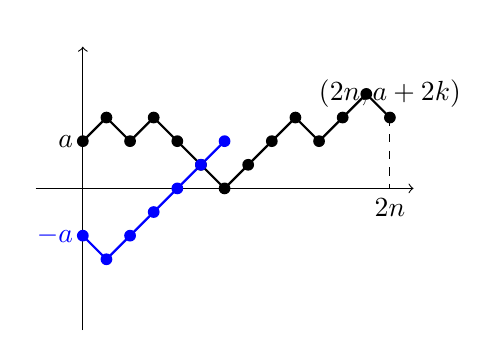
\begin{tikzpicture}[scale=0.6]
\draw[->] (0, -3) -- (0, 3) node[above] {};
\draw[->] (-1, 0) -- (7, 0) node[right] {};

\draw[thick] (0,1) -- (0.5, 1.5) -- (1, 1) -- (1.5, 1.5) -- (2, 1) -- (2.5, 0.5) -- (3, 0) -- (3.5, 0.5) -- (4, 1) -- (4.5, 1.5) -- (5, 1) -- (5.5, 1.5) -- (6, 2) -- (6.5, 1.5);
\draw[dashed] (6.5, 1.5) -- (6.5, 0);

\draw[blue, thick] (0,-1) -- (0.5, -1.5) -- (1, -1) -- (1.5, -0.5) -- (2, 0) -- (2.5, 0.5) -- (3, 1);

\node at (0,1) [left] {$a$};
\node at (0,-1) [left, blue] {$-a$};
\node at (6.5, 0) [below] {$2n$};
\node at (6.5, 1.5) [above] {$(2n, a+2k)$};

\foreach \point in {(0,1), (0.5, 1.5), (1, 1), (1.5, 1.5), (2, 1), (2.5, 0.5), (3, 0), (3.5, 0.5), (4, 1), (4.5, 1.5), (5, 1), (5.5, 1.5), (6, 2), (6.5, 1.5)}
    \node at \point [circle, fill, inner sep=1.5pt] {};

\foreach \point in {(0,-1), (0.5, -1.5), (1, -1), (1.5, -0.5), (2, 0), (2.5, 0.5), (3, 1)}
    \node at \point [circle, fill=blue, inner sep=1.5pt] {};
\end{tikzpicture}

Each path $(0, -a) \rightarrow (2n, a + 2k)$ consists of $n + a + k$ steps going
Northeast and $n - a - k$ steps going Southeast. The number of such
paths is $\binom{2n}{n+a+k}$.
\end{block}

\end{frame}

\begin{frame}
\frametitle{Splitting ballot sequences}
\begin{block}{Lemma}
Each nonempty ballot sequence splits uniquely into a concatenation
of the form
\[
    + \langle \text{ballot sequence} \rangle - \langle \text{ballot sequence} \rangle.
\]
\end{block}

\begin{block}{Proof}
\begin{center}
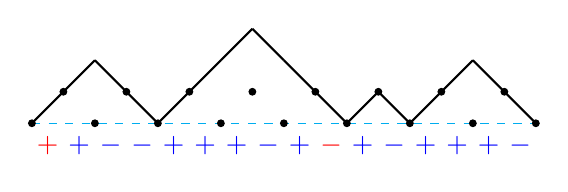
\begin{tikzpicture}[scale=0.4]
\draw[thick] (0,0) -- (1,1);
\draw[thick] (1,1) -- (2,2);
\draw[thick] (2,2) -- (3,1);
\draw[thick] (3,1) -- (4,0);
\draw[thick] (4,0) -- (5,1);
\draw[thick] (5,1) -- (6,2);
\draw[thick] (6,2) -- (7,3);
\draw[thick] (7,3) -- (8,2);
\draw[thick] (8,2) -- (9,1);
\draw[thick] (9,1) -- (10,0);
\draw[thick] (10,0) -- (11,1);
\draw[thick] (11,1) -- (12,0);
\draw[thick] (12,0) -- (13,1);
\draw[thick] (13,1) -- (14,2);
\draw[thick] (14,2) -- (15,1);
\draw[thick] (15,1) -- (16,0);

\draw[dashed, color=cyan] (0,0) -- (16,0);

\foreach \x in {0,1,2,3,4,5,6,7,8,9,10,11,12,13,14,15,16}
    \filldraw[fill=black, draw=black] (\x, {mod(\x,2)}) circle (3pt);

\node[red] at (0.5, -0.7) {$+$};
\node[blue] at (1.5, -0.7) {$+$};
\node[blue] at (2.5, -0.7) {$-$};
\node[blue] at (3.5, -0.7) {$-$};
\node[blue] at (4.5, -0.7) {$+$};
\node[blue] at (5.5, -0.7) {$+$};
\node[blue] at (6.5, -0.7) {$+$};
\node[blue] at (7.5, -0.7) {$-$};
\node[blue] at (8.5, -0.7) {$+$};
\node[red] at (9.5, -0.7) {$-$};
\node[blue] at (10.5, -0.7) {$+$};
\node[blue] at (11.5, -0.7) {$-$};
\node[blue] at (12.5, -0.7) {$+$};
\node[blue] at (13.5, -0.7) {$+$};
\node[blue] at (14.5, -0.7) {$+$};
\node[blue] at (15.5, -0.7) {$-$};
\end{tikzpicture}
\end{center}

Identify the first partial sum that is equal to 0.
\end{block}

\begin{block}{Theorem}
\[
    C_n = \sum_{k+\ell=n-1} C_k C_\ell.
\]
\end{block}
\end{frame}

\begin{frame}
\frametitle{Generating function for the Catalan numbers}

\begin{block}{Theorem/Exercise}
\[
\sum_{n=0}^{\infty} C_n x^n = \frac{1-\sqrt{1-4x}}{2x}.
\]
\end{block}

\begin{block}{Hint}
Use the recurrence
\[
C_n = \sum_{k+\ell=n-1} C_k C_\ell.
\]
This theorem can also be deduced from Newton's binomial theorem.
\end{block}

\end{frame}

\begin{frame}
Watch my video

\begin{center}
\begin{minipage}{0.8\textwidth}
\begin{align*}
    C_n &= \frac{1}{n+1}\binom{2n}{n} \\
    &= 1, 1, 2, 5, 14, 42, \dots
\end{align*}
\end{minipage}
\end{center}

\bigskip
\begin{itemize}
    \item[] Some illustrations appear here (a binary tree, a path, a polyhedron).
\end{itemize}
\bigskip

\begin{itemize}
    \item[] \url{https://www.youtube.com/watch?v=TAuJV5eNKLM}
    \item[] Beware: I make a serious algebra mistake when deriving the formula for the Catalan numbers.
\end{itemize}

\end{frame}

\begin{frame}
\frametitle{Ballot sequences}

\begin{block}{Definition}
A \alert{ballot sequence} of length $2n$ is a sequence of $n$ pluses and $n$ minuses in which each initial segment contains at least as many pluses as minuses.

\bigskip

\centering
\begin{tabular}{ccccc}
$ \begin{array}{|c|c|c|c|c|c|} \hline
+ & + & + & - & - & - \\ \hline
\end{array} $
&
$ \begin{array}{|c|c|c|c|c|c|c|} \hline
+ & + & - & + & - & + & - \\ \hline
\end{array} $
&
$ \begin{array}{|c|c|c|c|c|c|c|} \hline
+ & + & - & + & + & - & - \\ \hline
\end{array} $
&
$ \begin{array}{|c|c|c|c|c|c|c|} \hline
+ & - & + & + & - & + & - \\ \hline
\end{array} $
&
$ \begin{array}{|c|c|c|c|c|c|c|} \hline
+ & - & + & - & + & - & + \\ \hline
\end{array} $
\end{tabular}

\bigskip

Interpreting each $ \begin{array}{|c|} \hline
+ \\ \hline
\end{array} $ as 1 and each $ \begin{array}{|c|} \hline
- \\ \hline
\end{array} $ as -1, a ballot sequence is a sequence $(a_1,\dots,a_{2n})$ such that
\begin{itemize}
    \item each component $a_i$ is equal to either 1 or -1,
    \item $a_1 + \dots + a_{2n} = 0$, and
    \item each partial sum $a_1 + \dots + a_i$ is nonnegative.
\end{itemize}
\end{block}

\begin{block}{Theorem}
The number of ballot sequences of length $2n$ is $C_n$.
\end{block}

The proof will rely on the following lemma.
\end{frame}

\begin{frame}
\frametitle{Catalan numbers and circular arrangements}

\begin{center}
\begin{tabular}{c | c | c | c | c | c | c | c | c | c | c}
$n$ & 0 & 1 & 2 & 3 & 4 & 5 & 6 & 7 & 8 & 9 \\ \hline
$C_n$ & 1 & 1 & 2 & 5 & 14 & 42 & 132 & 429 & 1430 & 4862
\end{tabular}
\end{center}

\vspace{0.5cm}

\begin{block}{Theorem}
The number of circular arrangements of $n+1$ pluses and $n$ minuses, up to rotation, is the Catalan number $C_n$.
\end{block}

\vspace{0.2cm}

\begin{block}{Example: $n=3$}
\begin{center}
% Illustration Placeholder - Recreate the circles with +/- signs using TikZ if desired.
\begin{tabular}{cccc}
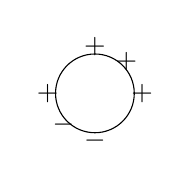
\begin{tikzpicture}[scale=0.5]
\draw (0,0) circle (1cm);
\node at (0,1.2) {$+$};
\node at (0,-1.2) {$-$};
\node at (1.2,0) {$+$};
\node at (-1.2,0) {$+$};
\node at (0.8,0.8) {$+$};
\node at (-0.8,-0.8) {$-$};
\end{tikzpicture}
&
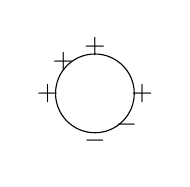
\begin{tikzpicture}[scale=0.5]
\draw (0,0) circle (1cm);
\node at (0,1.2) {$+$};
\node at (0,-1.2) {$-$};
\node at (1.2,0) {$+$};
\node at (-1.2,0) {$+$};
\node at (-0.8,0.8) {$+$};
\node at (0.8,-0.8) {$-$};
\end{tikzpicture}
&
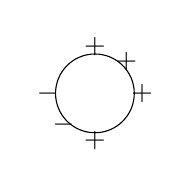
\begin{tikzpicture}[scale=0.5]
\draw (0,0) circle (1cm);
\node at (0,1.2) {$+$};
\node at (0,-1.2) {$+$};
\node at (1.2,0) {$+$};
\node at (-1.2,0) {$-$};
\node at (0.8,0.8) {$+$};
\node at (-0.8,-0.8) {$-$};
\end{tikzpicture}
&
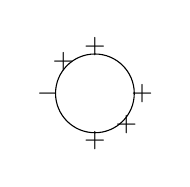
\begin{tikzpicture}[scale=0.5]
\draw (0,0) circle (1cm);
\node at (0,1.2) {$+$};
\node at (0,-1.2) {$+$};
\node at (1.2,0) {$+$};
\node at (-1.2,0) {$-$};
\node at (-0.8,0.8) {$+$};
\node at (0.8,-0.8) {$+$};
\end{tikzpicture}
\end{tabular}
\end{center}
\end{block}

\vspace{0.2cm}

\begin{block}{Proof}
To obtain the formula $\frac{1}{2n+1}\binom{2n+1}{n}$ for the number in question, use the Division Principle together with the fact that $\gcd(n, n+1) = 1$.
\end{block}

\end{frame}

\begin{frame}
\frametitle{Discrete Taylor's formula (2)}

\begin{block}{Example: $h_n = n^3$}
\begin{center}
\begin{tabular}{ccccccccc}
0 & 1 & 8 & 27 & 64 & 125 & 216 & 343 & $\cdots$ \\
& 1 & 7 & 19 & 37 & 61 & 91 & 127 & $\cdots$ \\
& & 6 & 12 & 18 & 24 & 30 & 36 & $\cdots$ \\
& & & 6 & 6 & 6 & 6 & 6 & $\cdots$ \\
& & & & 0 & 0 & 0 & 0 & $\cdots$ \\
& & & & & 0 & 0 & 0 & $\cdots$ \\
\end{tabular}
\end{center}

\begin{center}
$n^3 = \binom{n}{1} + 6 \binom{n}{2} + 6 \binom{n}{3}.$
\end{center}

\end{block}

\end{frame}

\begin{frame}
\frametitle{Catalan numbers}

\begin{block}{Definition}
The \textit{Catalan numbers} $C_n$ are defined by
\[
C_n = \frac{1}{n+1} \binom{2n}{n} = \frac{(2n)!}{n! (n+1)!} = \frac{1}{2n+1} \binom{2n+1}{n}.
\]
\end{block}

\begin{center}
\begin{tabular}{c | c | c | c | c | c | c | c | c | c | c}
$n$ & 0 & 1 & 2 & 3 & 4 & 5 & 6 & 7 & 8 & 9 \\
\hline
$C_n$ & 1 & 1 & 2 & 5 & 14 & 42 & 132 & 429 & 1430 & 4862
\end{tabular}
\end{center}

These numbers enumerate many families of combinatorial objects.

\end{frame}

\begin{frame}
\frametitle{Extrapolation of polynomials (1)}

Recall: a sequence $(h_n)$ is given by a polynomial in $n$ of degree $< k$ if and only if its $k$'th differences vanish. Application: \textcolor{blue}{extrapolation}.

\bigskip
\textbf{Problem}

Extrapolate a cubic polynomial $f(x)$ given the following values:
\begin{center}
\begin{tabular}{c||c|c|c|c}
$x$ & $a$ & $a+\delta$ & $a+2\delta$ & $a+3\delta$ \\
\hline
$f(x)$ & $1$ & $-2$ & $-5$ & $4$
\end{tabular}
\end{center}

\bigskip
\textbf{Solution}

Let us build a difference table for the sequence $h_n = f(a + n\delta)$.

The bottom entry 12 is \textcolor{blue}{replicated in the bottom row [why?]}.

Then the table is \textcolor{blue}{constructed bottom-up, column by column}.

\bigskip

\begin{center}
\begin{tabular}{rrrrrr}
$1$ & $-2$ & $-5$ & $4$ & \textcolor{blue}{$37$} & \textcolor{blue}{$106$} \\
 & $-3$ & $-3$ & $9$ & \textcolor{blue}{$33$} & \textcolor{blue}{$69$} \\
 &  & $0$ & $12$ & \textcolor{blue}{$24$} & \textcolor{blue}{$36$} \\
 &  &  & $12$ & \textcolor{cyan}{$\longrightarrow 12$} & \textcolor{cyan}{$\longrightarrow 12$}
\end{tabular}
\end{center}

\end{frame}

\begin{frame}
\begin{center}
Math 465: Introduction to Combinatorics

\vspace{1cm}

Andrew Sack

\vspace{2cm}

\hrulefill

\vspace{0.5cm}

Homework \#4 will be due Monday evening.

\vspace{0.5cm}

\hrulefill

\vspace{1cm}

These slides will be posted on Canvas.
\end{center}
\end{frame}

\begin{frame}
\frametitle{Extrapolation of polynomials (2)}

\begin{center}
\begin{tabular}{cccccccc}
    \fbox{1} & & $-2$ & & $-5$ & & $4$ & & $37$ & & $106$ \\
     & \fbox{$-3$} & & $-3$ & & $9$ & & $33$ & & $69$ \\
      & & \fbox{$0$} & & $12$ & & $24$ & & $36$ \\
       & & & \fbox{$12$} & & $12$ & & $12$ \\
\end{tabular}
\end{center}

\begin{block}{Remark/Exercise}
We did not need an explicit formula for this cubic polynomial in order to extrapolate it. If needed, such a formula can be written using the leftmost entries in the rows of the difference table, as follows:
\begin{align*}
    h_n &= \binom{n}{0} - 3\binom{n}{1} + 12\binom{n}{3} \\
    &= 1 - 3n + 2n(n-1)(n-2) \\
    &= 2n^3 - 6n^2 + n + 1.
\end{align*}
\end{block}

\end{frame}

\begin{frame}
Discrete Taylor's formula (1)
\end{frame}

\begin{frame}
Passing to the difference sequence is analogous to differentiation.

Let $\hat{h}_0, \hat{h}_1, \hat{h}_2,...$ be the leftmost entries in the difference table for $(h_n)$.

They are the analogues of the derivatives of a function at 0.
\end{frame}

\begin{frame}
\textbf{Proposition/Exercise}

The leftmost entries of the difference table are the coefficients in the expansion of $h_n$ in terms of binomial coefficients $\binom{n}{m}$:
\[
h_n = \sum_m \hat{h}_m \binom{n}{m} = \sum_m \frac{\hat{h}_m}{m!} \cdot (n)_m
\]
\end{frame}
\end{document}